\documentclass{article}






\usepackage{floatrow}
% Table float box with bottom caption, box width adjusted to content
\newfloatcommand{capbtabbox}{table}[][\FBwidth]
\usepackage{caption}
\usepackage{subcaption}
\captionsetup{compatibility=false}



\usepackage{array}
% For tabulars
\newcolumntype{P}[1]{>{\centering\arraybackslash}p{#1}}

\usepackage{pdfpages}
\usepackage{graphicx}
\usepackage{longtable}
%\usepackage[export]{adjustbox}
%\usepackage{tabu}
\usepackage{xcolor,colortbl}
\usepackage{caption}
\usepackage{subcaption}
\usepackage{float}

\usepackage{amsthm}

\usepackage[margin=0.65in]{geometry}

\begin{document}

\vspace*{3ex}
\begin{flushright}
{\large 10 November 2015}
\end{flushright}

\vskip20ex
\hskip3cm

\begin{center}


\begin{figure}[H]
\centering
\begin{subfigure}{.5\textwidth}
  \centering
  
\includegraphics[width=.9\linewidth]{images/mini.png}
\end{subfigure}%
\begin{subfigure}{.5\textwidth}
  \centering
  
\includegraphics[width=.9\linewidth]{images/pw.jpg}
\end{subfigure}
\end{figure}




\Large {\bf
	Bachelor Thesis \\
	Finite Automata for Pattern Recognition
}

\Large {\bf 
	Technical Project
}
\end{center}
\vskip2ex


\vskip25ex

\begin{flushleft}
{\large Bartlomiej Dybisz \\
Jakub Ciecierski

}
\end{flushleft}

\newpage
\tableofcontents
\newpage

%------------------------------------------------------------------------------

\section*{Document metric}

\begin{center}


\begin{table}[h]
\hspace*{-1.1cm}
\large
\begin{tabular}{|
>{\columncolor[HTML]{C0C0C0}}l |l|l|l|l|l|}
\hline
\multicolumn{6}{|l|}{\cellcolor[HTML]{C0C0C0}Document metric}                                                                                                                                         \\ \hline
Project:       & \multicolumn{2}{l|}{Finite automata for pattern recognition} & 
\cellcolor[HTML]{C0C0C0}Company: & \multicolumn{2}{l|}{WUT}                                               \\ \hline
Name:          & \multicolumn{5}{l|}{Technical Project}                                                                                                                                       \\ \hline
Topics:        & \multicolumn{5}{l|}{Architecture and algorithms defining the project}                                                                                                                                       \\ \hline
Author:        & \multicolumn{5}{l|}{Jakub Ciecierski, Bartlomiej Dybisz}                                                                                                                                                \\ \hline
File:          & \multicolumn{5}{l|}{technical\_project.pdf}                                                                                                                                      \\ \hline
Version no:    & 0.1                                                                      & \cellcolor[HTML]{C0C0C0}Status:  & Under development & \cellcolor[HTML]{C0C0C0}Opening date: & 2015-10-27 \\ \hline
Summary:       & \multicolumn{5}{l|}{Technical side of research on pattern recognition by finite automata}                                                                                                           \\ \hline
Authorized by: & \begin{tabular}[c]{@{}l@{}}Wladyslaw Homenda\end{tabular} & \multicolumn{3}{l|}{\cellcolor[HTML]{C0C0C0}Last modification date:}                         & 2015-11-10 \\ \hline
\end{tabular}
\end{table}

\end{center}



\section*{History of changes}

\begin{center}


\begin{table}[h]
\hspace*{-1.0cm}
\large
\begin{tabular}{|l|l|l|l|}
\hline
\multicolumn{4}{|l|}{\cellcolor[HTML]{C0C0C0}History of Changes} \\ \hline
Version         & Date         & Who        & Description        \\ \hline

0.1         
& 2015-11-10
& Jakub Ciecierski, Bartlomiej Dybisz
& Definition of the main purpose of the document       \\ \hline
\end{tabular}
\end{table}

\end{center}


%---------------------------------------------------------------

\section*{Schedule}

\begin{center}


\begin{table}[h]

\large
\begin{tabular}{|l|l|l|}
\hline
\multicolumn{3}{|l|}{\cellcolor[HTML]{C0C0C0}Schedule} \\ \hline
Date         & Note        & Planned Progress          \\ \hline
\hline

27.10.2015   & Lab1    & Presentation of Business Analysis   \\ \hline
03.11.2015   &    & Additional changes of Business Analysis   \\ \hline
7-9.11.2015   &     & First drafts of UML of particular modules   \\ \hline
14-16.11.2015   &     & Requirements analysis, design of algorithms and further UML development \\ \hline
17.11.2015   &  Lab2   & Presentation of Technical Analysis   \\ \hline
20-22.11.2015   &     & Implementation of mudules needed for testing and basic GUI   \\ \hline
31.11.2015   & Lab3    & Presentation of results of tests on synthetic and semi-synthetic data  \\ \hline
4-6.12.2015   &     & GUI and console application development  \\ \hline
15.12.2015   & Lab4    & Final GUI  \\ \hline
-------  & -------    & Work depends on acquired results  \\ \hline
08.01.2015  & Lab5    & Complete system presentation  \\ \hline
\end{tabular}
\end{table}

\end{center}


%---------------------------------------------------------------
\newpage




%---------------------------------------------------------------
\section{Production Model}
{\bf Waterfall} model is a model which was developed for software development; that is to create software. It is called as such because the model develops systematically from one phase to other in a downward fashion, like a waterfall.

{\color{red} NICE DECRIPTION LOL}

\begin{center}

	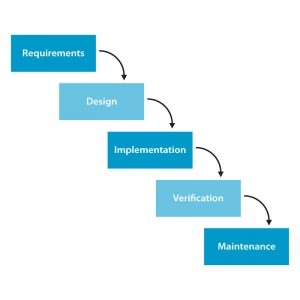
\includegraphics[width=80mm]{images/waterfall_model.jpg}

\end{center}


%---------------------------------------------------------------
\section{Technology}

%---- JC ----%


%---- BD ----%



\newpage




%---------------------------------------------------------------------
\section{Preliminaries}\label{sec:prelim}



%---------------------------------------------------------------------
%---------------------------------------------------------------------
\subsection{Hamming Distance} \label{sec:hamming}

%\begin{definition}
Hamming distance $H_d$ between two string of the same length is the number of positions at which the corresponding symbols differ.
%\end{definition}

%\begin{example} 
Let $w = John$ and $v = Jhon$. Notice that the symbols at positions two and three differ. Thus the Hamming distance between these two strings is $H_d(w,v) = 2$.
%\end{example}

%---------------------------------------------------------------------
%---------------------------------------------------------------------
\subsection{Clustering} \label{sec::cluster}

Clustering is a method of segregating elements of a given data set into groups. Elements similar to each other should fall into one group while dissimilar elements are supposed to be separated.

The problem arises when no prior information about the structure of the data is given. 

%---------------------------------------------------------------------
%---------------------------------------------------------------------
%---------------------------------------------------------------------
\subsubsection{K-Means}

The well known k-means algorithm is employed for clustering. Let's assume that a~data set $X$ of size $n$ is going to be partitioned into $k$ number of clusters and each element $x_{j}\in X$ is assigned a~cluster. In order to do that, we find cluster centers $\mu_{i}, i=1,\ldots,k$ that minimize the distance from the elements from data set. Formally k-means solves the following optimization problem:
%\begin{equation}
%  $\argmin_{C}\sum_{i=1}^{k}\sum_{x\in C_{i}} d(x,\mu_{i})$
%\end{equation}
where $C_{i}$ is the set of elements that correspond to $i$-th cluster and $d(x,\mu_{i})$ is a~chosen distance measure between element $x$ and the cluster center $\mu_{i}$. At the first stage of the algorithm k centers $\mu_{i}$ are selected. Then each element is assigned to the closest cluster. The centers are updated with the mean of all points belonging to the corresponding cluster
\begin{equation}
  \mu_{i} = \frac{1}{|C_{i}|} \sum_{x\in C_{i}} x
\end{equation}

This process is repeated until convergence. It is worth mentioning that k-means might not find the best possible 
configuration.


%---------------------------------------------------------------------
%---------------------------------------------------------------------
%---------------------------------------------------------------------
\subsubsection{Cluster Evaluation}

%---------------------------------------------------------------------
%---------------------------------------------------------------------
\subsection{Automaton} \label{sec:autom}
%\begin{definition}
Automaton is a system of five fields:
\begin{center}
	$A = (Q, \Sigma, \delta, q_0, F)$
\end{center}

where \\
$Q$ - finite set of states. \\
$\Sigma$ - Finite input alphabet. \\
$\delta$ - transition function. $\delta: Q \times \Sigma \rightarrow Q$ \\
$q_0$ - the initial state. $q_0 \in Q$ \\
$F$ - Set of accepting states. $F \subseteq Q$ \\
%\end{definition}

Table~\ref{fig:ttable_std} shows transition table for an example of an automaton.

%%%
%
% Standard Transition function
%
%%%
\begin{figure}
\CenterFloatBoxes
\begin{floatrow}

\ttabbox
  {
  \centering
  \setlength{\tabcolsep}{15pt}
	\renewcommand{\arraystretch}{1.5}
	\begin{tabular}{|P{1.0cm} || P{0.6cm} | P{0.6cm} |}
	\hline
	$\delta$ & a & b \\
	\hline
	\hline
	$\rightarrow q^-$ 		& $q_0$ & $q_1$ \\
	\hline
	$q_0 \rightarrow$ 		& $q_R$ & $q_R$ \\
	\hline
	$q_1 \rightarrow$ 		& $q_1$ & $q_1$ \\
	\hline
	$q_R$  					& $q_R$ & $q_R$ \\
	\hline
	\end{tabular}
  }
  {\caption{Transition table for A with $\delta: Q \times \Sigma \rightarrow Q$}\label{fig:ttable_std}}

\ffigbox
  {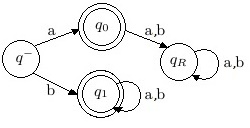
\includegraphics[width=0.35\textwidth]{images/automaton_example.jpg}}
  {\caption{Example of Automaton A}\label{fig:automaton_ex}}
\killfloatstyle

\end{floatrow}
\end{figure}


The binary representation of automaton might perhaps provide more adequate solution for a computer. Thus a new transition function is defined, $\delta^{'}: Q \times \Sigma \times Q \rightarrow \{0,1\}$. It simply provides an answer whether there exists a transition between two states for a given symbol. For example, by looking at figure~\ref{fig:ttable_std} we can define value for $\delta^{'}(q^-,a,q^0) = 1$, since there exists a transition from $q^-$ to $q^0$ through symbol $a$. The entire automaton is presented in figure~\ref{fig:ttable_bin}.


%%%
%
% Binary transition function.
%
%%%
\begin{figure}
\begin{center}

	\setlength{\tabcolsep}{4pt}
	\renewcommand{\arraystretch}{1.4}
	
	\begin{subfigure}{.5\textwidth}

	\centering
	\begin{tabular}{|P{1.0cm} || P{0.8cm} | P{0.8cm} | P{0.8cm} | P{0.8cm}|}

	\hline
	a & $\rightarrow q^-$ & $q_0 \rightarrow$ & $q_1 \rightarrow$ & $q_R$ \\
	\hline
	\hline
	$\rightarrow q^-$ 		& $0$ & $1$ & $0$ & $0$ \\
	\hline
	$q_0 \rightarrow$ 		& $0$ & $0$ & $0$ & $1$ \\
	\hline
	$q_1 \rightarrow$ 		& $0$ & $0$ & $1$ & $0$ \\
	\hline
	$q_R$  					& $0$ & $0$ & $0$ & $1$ \\
	\hline

	\end{tabular}

	\caption{Transition table for symbol $a$}
	\label{fig:ttable_bin_a}	
	
	\end{subfigure}%
	\begin{subfigure}{.5\textwidth}
	
	\centering
	\begin{tabular}{|P{1.0cm} || P{0.8cm} | P{0.8cm} | P{0.8cm} | P{0.8cm}|}
	
	\hline
	b & $\rightarrow q^-$ & $q_0 \rightarrow$ & $q_1 \rightarrow$ & $q_R$ \\
	\hline
	\hline
	$\rightarrow q^-$ 		& $0$ & $0$ & $1$ & $0$ \\
	\hline
	$q_0 \rightarrow$ 		& $0$ & $0$ & $0$ & $1$ \\
	\hline
	$q_1 \rightarrow$ 		& $0$ & $0$ & $1$ & $0$ \\
	\hline
	$q_R$  					& $0$ & $0$ & $0$ & $1$ \\
	\hline

	\end{tabular}
	
	\caption{Transition table for symbol $b$}
	\label{fig:ttable_bin_b}
	
	\end{subfigure}%

	
\caption{Transition tables for symbols $a$ and $b$, making up the entire transition function $\delta^{'}: Q \times \Sigma \times Q \rightarrow \{0,1\}$}

\label{fig:ttable_bin}
\end{center}
\end{figure}

It is important to note that to preserve determinism, there must exist exactly one transition from any state for a given symbol. In other words in each transition table for $\delta^{'}$ a single row must be a sequence of $0s$ and a single digit $1$.

%---------------------------------------------------------------------
%---------------------------------------------------------------------
%---------------------------------------------------------------------
\subsubsection{Decoding} \label{sec:auto_dec}

Let us denote the number of states by $n = |Q|$, and number of symbols in alphabet by $r = |\Sigma|$. Further, we shall enumerate all states 	$Q = \{q_1, q_2, \ldots, q_n\}$, and all the symbols in the alphabet 	$\Sigma = \{x_1, x_2, \ldots, x_r\}$. We will also define the size of automaton $s(A) = n*r$.

We now turn to the binary approach of transition function $\delta^{'}$ described in the figure~\ref{fig:ttable_bin}. Notice that each table for symbol $x_l$ for $l = 1,2, \dots, r$ has exactly $n$ rows. Furthermore, we can easily decode each $row_{x_l, i}$ into a natural number. Let $j$ be the index of occurrence of digit $1$ in the $row_{x_l, i}$. The natural number $j$ will then be a decoding of $row_{x_l, i}$. Decoding of a single table will be a vector of $n$ natural numbers. Notice that the first element of such vector will correspond to the transition of initial state. Now the last objective of representing the automaton is to combine all vectors, each corresponding to transition table for symbol $x_{l}$. We simply append all vectors in order of the symbols' enumeration. The entire proceeder is illustrated in figure~\ref{fig:encoding}. Firstly, in figures~\ref{fig:encoding_a} and~\ref{fig:encoding_b} we see decoding of transition tables for symbols $a$ and $b$ respectively. Finally the figure~\ref{fig:encoding_both} shows entire decoding of automaton $A$. We will call such decoding a direct or natural decoding of automaton with binary transition function.

%%%
%
% Natural encoding
%
%%%
\begin{figure}
\begin{center}

	\setlength{\tabcolsep}{1pt}
	\renewcommand{\arraystretch}{1.9}
	
	\begin{subfigure}{.5\textwidth}
	\centering
	
	\begin{tabular}{|P{.9cm} | P{0.9cm} | P{0.9cm} | P{0.9cm} | P{0.9cm} |}
	\hline
	$r_{a,1}$  & $r_{a,2}$ & $r_{a,3}$ & $r_{a,4}$ \\
	\hline
	\hline
	$2$  & $4$ & $3$ & $4$ \\
	\hline	
	\end{tabular}
\caption{Natural decoding of Transition table \\presented in figure~\ref{fig:ttable_bin_a}}
	\label{fig:encoding_a}
	\end{subfigure}%
	\begin{subfigure}{.5\textwidth}
	\centering
	
	\begin{tabular}{|P{.9cm} | P{0.9cm} | P{0.9cm} | P{0.9cm} | P{0.9cm} |}
	\hline
	$r_{b,1}$  & $r_{b,2}$ & $r_{b,3}$ & $r_{b,4}$ \\
	\hline
	\hline
	$3$  & $4$ & $3$ & $4$ \\
	\hline	
	\end{tabular}
	\caption{Natural decoding of Transition table \\presented in figure~\ref{fig:ttable_bin_b}}
	\label{fig:encoding_b}
	\end{subfigure}
	
	\begin{subfigure}{.5\textwidth}
	\centering
	
	\begin{tabular}{|P{.9cm} | P{0.9cm} | P{0.9cm} | P{0.9cm} | P{0.9cm} |P{.9cm} | P{0.9cm} | P{0.9cm} | P{0.9cm} | P{0.9cm} |}
	\hline
	$r_{a,1}$  & $r_{a,2}$ & $r_{a,3}$ & $r_{a,4}$ & $r_{b,1}$  & $r_{b,2}$ & $r_{b,3}$ & $r_{b,4}$ \\
	\hline
	\hline
	$2$  & $4$ & $3$ & $4$ & $3$  & $4$ & $3$ & $4$ \\
	\hline	
	\end{tabular}
	\caption{Natural decoding of all Transition tables presented in figure~\ref{fig:ttable_bin}. The abbreviation $r_{x,i}$, represents the $i$-th row of table corresponding to symbol x}
	\label{fig:encoding_both}
	\end{subfigure}

\caption{Natural decoding of Automaton A}
\label{fig:encoding}
\end{center}
\end{figure}

Natural decoding of an automaton with $n$ states and $r$ symbols in the alphabet will be a vector of size $n*r$. First element of each sub vector will indicate the transition for initial symbol. The retrieval of elements corresponding to transitions of specific symbols is omitted due to its triviality.

Formally, each element of the decoding vector is a natural number greater than 0. Summarizing, the elements of each dimension, take values from the discrete set $\{1,2, \ldots, n\}$.

It is worth mentioning, that in such decoding the information about accepting states is lost. This shall be of no concern, since the problem of this study takes no interest in actually accepted words. This discussion will resume in the following section.





%---------------------------------------------------------------
\section{Algorithms}

%---- JC ----%
\subsection{Particle Swarm Optimization}
In the Particle Swarm Optimization (PSO), originated by Eberhart and Kennedy in~\cite{pso_origin}, we look for optimal solution of the problem in the solution space. 

Each solution is called a particle and it consists of the following fields. First of all, the particle stores $fitness$ value which is evaluated by the fitness function, representing the quality of the solution and the best fitness value computed so far. It also stores the position $X_p$ and velocity vector $V_p$ which lets the particle travel through the solution space. Lastly two additional positions called $pbest_p$ and $lbest_p$ are stored. The position in which the particle $p$ reached its best fitness value so far is called $pbest_p$. However, the $lbest_p$ is the position of the best fitness value obtained so far by any other particle in the neighbourhood of particle $p$. The concept of neighbourhood is defined later in this section.

PSO is initialized with random group of particles. It then searches for the optimal solution by updating generations.
In each iteration $t$, the particles are updated by calculating new fitness and velocity which in turn is applied to update new position of the particle. $X_p(t)$ will denote the position of particle $p$ at time $t$, i.e. the $t$-th iteration. Similarly, the velocity vector is denoted by $V_p(t)$.

The PSO will take as input number of states $n$ and number of symbols in alphabet $r$.

Firstly, the general flow of the PSO algorithm is given, then each module is discussed and defined in details.

\begin{center}

\begin{enumerate}
	\item For the input $n$ and $r$, initialize the group of particles.

	\item For each particle: \label{itm:pso_iter}
	\begin{enumerate}
		\item Calculate the fitness value, using the fitness function.
		\item Compare the fitness to its best obtained so far, the better value is stored together with $pbest_p$	
		
		\item Update velocity and position.	
		
		\item Find neighbourhood and update $lbest_p$ position.
	\end{enumerate}		
	

	
	\item Repeat~\ref{itm:pso_iter}. until an ending criterion is met.

	\item Output the best solution	
	
\end{enumerate}

\end{center}

We now concentrate on describing in details each step of the PSO algorithm. The following part of this section is devoted to illustrating problems associated with the objective of this study and more importantly, methods of solving these problems.


%---------------------------------------------------------------------
%---------------------------------------------------------------------
%---------------------------------------------------------------------
\subsubsection{Representing the solution}
As an input, the PSO algorithm takes number of states $n$ and number of symbols in the alphabet $r$.
Solution that the PSO is trying to find is an automaton. Let us recall that automaton is a system: $A = (Q, \Sigma, \delta, q_0, F)$. In a single PSO instance we assume that a set of states $Q$ and alphabet $\Sigma$ is invariant. Through the nature of our problem we can conclude that distinguishing the set $F$ of accepting states is not necessary. Namely, the tool given to us (DFA) described in section~\ref{sub:definition} only answers whether any arbitrary two words are in the relation induced by the language. That information suffices in the process of recreating that DFA. Thus, we only need to represent the transition function and initial state.

The position of our particles will be represented by the natural decoding vector of size $n*r$ of an automaton described in section~\ref{sec:auto_dec} with more freedom allowed. Namely, all of the dimensions of the position will take real values in the interval $[1, n]$. Whenever we need to encode the automaton back, we simply round up the values, taking the closest integer value. The real number $3.4$ becomes $3$ and $3.5$ becomes 4.

As we may learn further in the article, the method of updating the particle will make a good use of continuous interval. On the other hand, the method of rounding up real numbers, might be vulnerable to error.



%---------------------------------------------------------------------
%---------------------------------------------------------------------
%---------------------------------------------------------------------
\subsubsection{Initialization}
In order to initialize the PSO algorithm, we must first decide on the size of the swarm (i.e. the number of particles). The swarm will be a static group, meaning that the size will not change through out the computations of a single PSO instance. The size should then be a constant value, in terms of an automaton given at the time. We propose that the size of the swarm should be proportional to the size of the automaton. To be precise, the swarm size is equal to the size of the automaton times a constant $c_P$ called a $population$ factor.

Further, we must initialize particle's position. Let us recall that the dimension of the search space is defined by the size of an automaton, namely $(n*r)$, where $n$ is the number of states and $r$ is the number of symbols in the alphabet. Each dimension taking a real value in the range $[1, n]$. Thus, we proceed to generate random position in the given range.

The initial velocities will be generated from the range $[-n,n]$. It is also crucial to define a maximum change in position that one particle can take during a single iteration. For this purpose the constant $v_{max}$ is defined that prevents the particle from travelling in any dimension further than $v_{max}$ units. The maximum change is defined by the equation 

\begin{equation}
	v_{max} = (\frac{n}{2})c_{v}
\end{equation}
where $c_{v}$ is a constant $speed$ factor and $v_{max} \leq n$.

In all cases uniform distribution is used for random number generation.

%---------------------------------------------------------------------
%---------------------------------------------------------------------
%---------------------------------------------------------------------
\subsubsection{Fitness Function}\label{sec:fitness}
It describes how well a particle (in our case an automaton) reflects the goal. Since all we know about our target DFA (accepting language $L$) is a tool described in subsection \ref{sub:definition}, we decided to base our fitness function on knowledge about relation $R_{L}$. 

Measure is fairly simple: for a given set of pairs of words, we check how many of them are correctly classified to equivalence class (using $R_{L} relation$) and divide this amount by number of all pairs. We will use example to illustrate the process.

%\begin{example}\label{ex:fitness}


Let us assume that we have following set of pairs
\[
S_{test} = \{(x_1,y_1), (x_2,y_2), (x_3, y_3), (x_4, y_4), (x_5, y_5)\} \subset \Sigma^{*}\times\Sigma^{*} 
\]
and an automaton $A_p$ (encoded back from a particle $p$).
Let us also recall automaton $T$, whose behaviour has been described in definition \ref{def:T} and define $\# = \{ x : x \in \{1 ,0 \}\}$  Having all of this we can construct simple table to illustrate the idea:

\begin{figure}[H]
\begin{center}
\begin{tabular}{ m{4.5em}  m{3em}  m{3em}  m{3em} }
                 & $T$ & $A_p$ & $\#$ \\  
 $x_1 R_{L} y_1$ & 1 & 0 & 0 \\   
 $x_1 R_{L} y_1$ & 0 & 0 & 1 \\   
 $x_1 R_{L} y_1$ & 0 & 0 & 1 \\   
 $x_1 R_{L} y_1$ & 1 & 1 & 1 \\   
 $x_1 R_{L} y_1$ & 0 & 0 & 0 \\   
\end{tabular}
\caption{Computing the error of an automaton $A_p$}
\label{fig:fitness_table}
\end{center}
\end{figure}

%\end{example}

Entries of figure \ref{fig:fitness_table} are calculate as follows:
\begin{enumerate}
\item Check computation of automaton $T$ for each pair of words from set $S_{test}$
\item If computations end in the same state for both words, put 1 in column $T$ and row corresponding to that pair.
\item Otherwise put 0
\item Repeat steps 1., 2. and 3. for automaton $A_p$ and write results in column $A_p$
\item If in row for (columns $T$ and $A_p$), we have the same digits (i.e. 1 1 or 0 0 ), put 1 in the last column ($\#$)
\item Otherwise put 0
\end{enumerate}

At this point we can define fitness function $F$, in terms of presented notation:
\[
	F = \frac{|\{x \in \# : x = 1 \}|}{|\#|}
\]



Concerning given example, $F = \frac{3}{5} = 0.6$. One needs to note that this function is never bigger than 1, nor less than 0. Closer $F$ gets to one, better the automaton approximation. 
%---------------------------------------------------------------------
%---------------------------------------------------------------------
%---------------------------------------------------------------------
\subsubsection{Updating the particle}


% Naive approach

%The naive approach of updating the particles' positions was proposed in the original PSO %algorithm~\cite{pso_origin}.

%\begin{equation}
%		V_p(t+1) = V_p(t) + c_1 * \mu_1 *(pbest_p - X_p(t)) + c_2 * \mu_2 *(lbest_p - X_p(t))
%	\end{equation}
%
%	\begin{equation}
%		X_p(t+1) = X_p(t) + V_p(t)
%	\end{equation}
%	where:\\
%	$c_1, c_2$ are the constant learning factors.\\
%	$\mu_1, \mu_2$ are random numbers in the range [0,1]. {\color{red} TODO What %distribution function - uniform ?} \\



The following method of updating the particles has its origins in the Standard Particle Swarm Optimization version 2011 presented in~\cite{pso_11}

Let $G_p(t)$ be the centre of gravity of the three points:
\begin{enumerate}
	\item Current position. \\
	$X_p(t)$
	
	\item Point a bit beyond $pbest_p$. \\
	$Y_{p1}(t) = c*(pbest_p-X_p(t))$
	
	\item Point a bit beyond $lbest_p$. \\
	$Y_{p2}(t) = c*(lbest_p-X_p(t))$
			
\end{enumerate}

The constant $c = \frac{1}{2} + ln(2)$ called a learning factor, together with the inertia parameter that weights the particle's velocity $\omega = \frac{1}{2 * ln(2)}$ used in further equations, was proposed by Clerc in~\cite{pso_anal}.

Formally $G_p(t)$ it is defined by the following formula 
\begin{equation}
	G_p(t) = \frac{X_p(t) + Y_{p1}(t) + Y_{p2}(t)} {3}
\end{equation}

We now define a random point $X^{'}_p$ in the hypersphere
\begin{center}
	$\mathcal{H}_p(G_p, d(G_p, X_p))$ 
\end{center}
of centre $G_p$ and of radius $d(G_p, X_p)$ where the function $d$ is an euclidean distance between two points. The time $t$ has been omitted for simplicity.

The velocity update is computed by
\begin{equation}
	V_p(t+1) = \omega * V_p(t) + X^{'}_p(t) - X_p(t)
\end{equation}
Thus the position is updated by the equation

\begin{equation}
	X_p(t+1) = \omega * V_p(t) + X^{'}_p(t)
\end{equation}

% Exploitation vs Exploration

%This method of updating the particles grants adequate definitions for $exploitation$ and $exploration$. Namely the exploitation occurs when $X_p(t+1)$ is inside atleast one hypersphere $\mathcal{H}_q$, otherwise we recognize exploration.


% Interval confinement
It may happen that the particle might leave the search space, in means that the particle lies outside the acceptable interval. If that happens we generally try to lead the particle back to its right course. For each dimension $x_{d} \in X_p$ that lies  outside the acceptable interval we apply the following:

  \[
	x_{d} \notin [x_{min}, x_{max}] \Rightarrow \left \{
                \begin{array}{ll}
                  v_{d} = 0 \\
                  x_d < x_{min} \Rightarrow x_d = x_{min} \\
                  x_d > x_{max} \Rightarrow x_d = x_{max}
                \end{array}
              \right.
  \]

This means that the corresponding dimension of velocity vector $v_d \in V_p$ is zeroed and the position is bound to the edge of the interval.

%---------------------------------------------------------------------
%---------------------------------------------------------------------
%---------------------------------------------------------------------
\subsubsection{Neighbourhood}
The neighbourhood system is defined by grouping the swarm into clusters. Cluster analysis methods can estimate the number of clusters $k$ that a data set should be grouped with. An algorithm for cluster evaluation used in this work is called mcclain-rao defined in~\cite{mc_rao}. Having the knowledge of data distortion, the data is then clustered into $k$ clusters, where each cluster represents a single neighbourhood. K-means algorithm is used to compute the clustering. The following formulates the algorithm for neighbourhood update.

\begin{enumerate}
	\item Evaluate number of clusters in the swarm using the mcclian-rao index. Denote that number by $k$.
	\item Group the swarm into $k$ clusters using k-means algorithm.
	\item Each cluster represents a single neighbourhood.
\end{enumerate}


%---------------------------------------------------------------------
%---------------------------------------------------------------------
%---------------------------------------------------------------------
\subsubsection{Ending criteria}
The computation finishes after $t_{max}$ iterations or after finding a satisfactory solution which is bounded by $F_{max} \in [0,1]$, where value 1 corresponds to trying to find the automaton exactly as good as $T$ defined in definition~\ref{def:T}.

%---- BD ----%


%---------------------------------------------------------------
%---------------------------------------------------------------
\subsubsection{Examples}
% Examples of algorithms, if any.

%---- JC ----%


%---- BD ----%

%---------------------------------------------------------------
\section{Data structures}

%---- JC ----%


%---- BD ----%

%---------------------------------------------------------------
\section{Modules}
	
%---- JC ----%


%---- BD ----%

%---------------------------------------------------------------
\section{Modelling}

%---- JC ----%


%---- BD ----%


\end{document}


